%In dit hoofdstuk moet het volgende besproken worden:
%-Uitleggen van het probleem
%-Hoe ik tewerk ga gaan
%-Gaan we concluderen met de onderzoeksvraag
\chapter{Situering}\label{hfdst:situering}
Televic Rail heeft een Python test framework ontworpen waarmee zij in staat zijn om verschillende producten te onderwerpen aan verschillende testscenario's.
Het framework werd ontworpen om gebruikt te worden op verschillende testtorens en werd later aangepast om bruikbaar te zijn op gewone computers.
Dit framework wordt intensief gebruikt tijdens het productieproces en is een spilfiguur voor het afleveren van producten die voldoen aan strenge veiligheidsnormen.

\section{Het probleem}\label{sec:probleem}
De applicatie gebruikt verschillende Python bibliotheken en hardware drivers om correct te functioneren.
Het installatieproces is tijdrovend en foutgevoelig.
Bij het uitbrengen bij een nieuwe versie van de applicatie, bijvoorbeeld bij het uitbrengen van een nieuwe driver, bibliotheek of om nieuwe producten te ondersteunen, moet de applicatie geüpdatet worden.
Dit proces lijdt aan dezelfde gebreken als het installatieproces.
Het doel van deze thesis is zoeken van een langdurige oplossing voor dit probleem.
Na een onderzoek zal een prototype geproduceerd worden die als oplossing aangeboden wordt aan het bedrijf.

%Packager
Een probleemanalyse onthulde al snel dat dit probleem onder te verdelen is in verschillende deelproblemen.
Het framework bestaat uit verschillende componenten, hieronder vallen de drivers en bibliotheken.
Elke component heeft een unieke installatiewijze en de componenten moeten in een specifieke volgorde geïnstalleerd worden.
Hiernaast moeten verscheidene componenten geconfigureerd worden aan de hand van een configuratiebestand.
Dit configuratiebestand is doelsysteem specifiek.
Tijdens het onderzoek zal er onderzocht welke technologieën gebruikt zal worden om al deze componenten te combineren tot één uitvoerbaar bestand.
Bij het selectieproces moet er rekening gehouden worden met de toekomst.
Er wordt best een technologie gekozen die cross-platform is, zodanig dat het bedrijf niet beperkt wordt in de toekomst.

%Server
De probleemanalyse onthulde ook dat de verschillende executables verspreidt moeten worden.
Door dit proces te automatiseren, is het mogelijk om waardevolle informatie te verzamelen.
Hiermee zouden rapporten gegeneerd kunnen worden voor het bedrijf.
Tijdens het ontwerpen zal schaalbaarheid een belangrijke factor spelen.
Naar de toekomst toe zal het aantal systemen waarop de applicatie geïnstalleerd wordt toenemen.

%Environment
Zoals reeds hierboven vermeld, is het installatieproces foutgevoelig.
Na de foutanalyse bleek dat hiervoor een schaalbare oplossing voor gevonden moet worden.
Bij het finaliseren van een component installatie, moeten de functionaliteiten van de component gecontroleerd worden.
Mocht deze incorrect functioneren dan moet een gepaste actie, eventueel een rollback, gebeuren. 
Ook na de volledige installatie moet gecontroleerd worden of het geheel correct functioneert.
Hierdoor wordt er voorkomen dat er nodeloos veel tijd verloren gaat in het herinstalleren van de applicatie.
Robuustheid zal een belangrijke component zijn tijdens de ontwerpfase.
Bij het ontwerpen moet gebruiksvriendelijkheid in het achterhoofd gehouden worden.

\section{Werkwijze}
In Sectie~\ref{sec:probleem} werd opgelijst wat de problemen zijn. 
In wat volgt zullen verschillende oplossingswijzes opgesomd worden met vervolgens de werkwijze.

Na de probleemanalyse werd het al snel duidelijk dat het werk op te delen valt in drie grote componenten.
Deze drie onderdelen zullen de basis vormen voor de architectuur en zullen gebruikt worden als leidraad.
Het eerste onderdeel zal bestaan uit een packager met als doel het inpakken van de nodige drivers, bibliotheken, ... .
Naast de packager is er een deployment server nodig die instaat voor het verspreiden van de installers die de packager aflevert.
Dankzij het automatiseren van de deployment, kan het installatieproces per client getrackt worden. %getrackt is juist
Om deze stap te vereenvoudigen, moet aan de client-side een deployment environment voorzien worden.
In die omgeving wordt de installatie geïsoleerd.
Mocht een rollback nodig zijn, dan kan deze op een eenvoudige manier gebeuren.

Gedurende deze thesis wordt een prototype ontworpen.
In Figuur~\vref{fig:overzichtsDiagram} wordt de algemene structuur van de applicatie weergegeven.
Met behulp van deze basis is het mogelijk om een demo te produceren die de verschillende problemen verhelpt.

\begin{figure}[!hbt]
\centering
  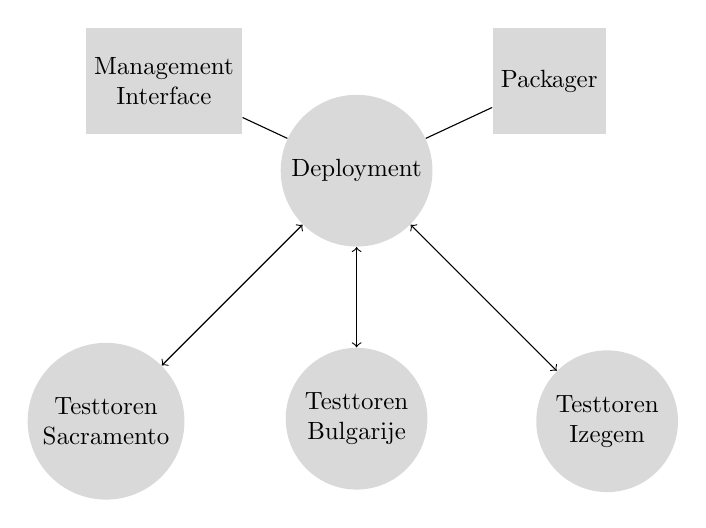
\begin{tikzpicture}[scale=.9, transform shape]
\tikzstyle{every node} = [circle, minimum size = 2cm, fill=gray!30]
\node (a) at (0, 0) {Deployment};
\node[shape = rectangle,minimum size = 1.5cm] (packager) at +(25: 3) {Packager};
\node[shape = rectangle,minimum size = 1.5cm, align=center] (logger) at +(155: 3) {Management\\ Interface};
\node[align=center] (b) at +(225: 5) {Testtoren\\ Sacramento};
\node[align=center] (c) at +(270: 3.5) {Testtoren\\ Bulgarije};
\node[align=center] (d) at +(315: 5) {Testtoren\\ Izegem};
\foreach \from/\to in {a/b, a/c, a/d}
\draw [<->] (\from) -- (\to);
\draw [-] (a) -- (packager);
\draw [-] (a) -- (logger);
\end{tikzpicture}
  \caption{Overzichtsdiagram van de algemene structuur}
  \label{fig:overzichtsDiagram}
\end{figure}

%In dit hoofdstuk\index{hoofdstuk} gaan we een voorbeeld geven van een voetnoot\footnote{Dit is dus een voetnoot}. Een referentie naar hoofdstuk ~\ref{verwijzing}, dat zich op pagina \pageref{verwijzing} bevindt, is dus ook een koud kunstje. Zorg er wel voor dat je de namen van de labels een beetje verstandig kiest. Hoofdstukken label je het best als hfdstk:naam, plaatjes als img:naam en tabellen\index{tabellen} als tabel:naam. Zo verlies je zelf de bomen in het bos niet.